\tikzstyle{feuille}=[draw, rectangle, inner sep = 0.12cm]
\tikzstyle{noeud}=[draw, rectangle,rounded corners, minimum width= 0.64cm, line width = 1pt]
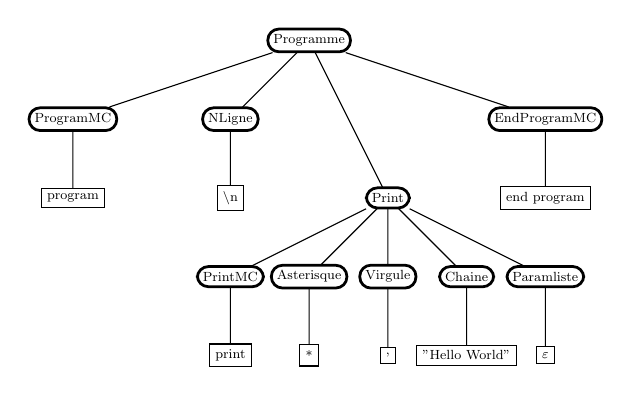
\begin{tikzpicture}[
        baseline=(base), 
        level/.style={sibling distance = 2cm/#1, level distance = 1cm},
        every node/.style={scale=0.6, font=\footnotesize}
    ]
    
    \node[ noeud] {Programme}
    child { 
        node[ noeud] (base) {ProgramMC}
        child { 
            node [ feuille] {program}
        }
    }
    child { 
        node[ noeud] {NLigne}
        child { 
            node [ feuille] {\textbackslash n}
        }
    }
    child [ level distance=2cm]{ 
        node [ noeud] {Print}
        child {
            node [noeud] {PrintMC}
            child { 
                node [ feuille] {print}
            }
        }
        child{
            node [noeud] {Asterisque}
            child { 
                node [feuille] {*}
            }
        }
        child{
            node [noeud] {Virgule}
            child { 
                node [feuille] {,}
            }
        }
        child{
            node [noeud] {Chaine}
            child { 
                node [feuille] {"Hello World"}
            }
        }
        child{
            node [noeud] {Paramliste}
            child { 
                node [feuille] {$\varepsilon$}
            }
        }
    }
    child { 
        node[ noeud] {EndProgramMC}
        child { 
            node [ feuille] {end program}
        }
    };

\end{tikzpicture}